\chapter{Theory}
\label{ch:theory}

This chapter is meant to provide the theoretical background necessary to understand the OVOS method and its implementation, and how we extend it to Quantum computing. The content is structured to build from fundamental concepts in electronic structure theory to the specific mathematical formulations used in OVOS. The chapter is structured in four sections: (\ref{sec:theory_elec_struct_prob}) the electronic structure problem and the importance of electron correlation, (\ref{sec:theory_wavefunction_methods}) the wavefunction methods that are the basis for OVOS, (\ref{sec:theory_background_ovos}) the mathematical framework for OVOS, and (\ref{sec:theory_relevance_qc}) the relevant aspects of OVOS on quantum computers. 

\section{The Electronic Structure Problem}
\label{sec:theory_elec_struct_prob}

The electronic structure problem is the task of solving the non-relativistic, time-independent Schrödinger equation for a system of N electrons moving in the electrostatic potential of M fixed nuclei, reflecting the Born-Oppenheimer approximation.\footnote{The Born-Oppenheimer approximation assumes that the nuclei are stationary due to their much larger mass compared to electrons, allowing the electronic and nuclear motions to be separated.}
Typically, the electronic system is expressed as the Schrödinger equation \cite{Helgaker2000}:
\begin{align}
    \label{eq:electronic_schrodinger}
    \hat{H}_{el} \Psi(\mathbf{r}_1, \mathbf{r}_2, \ldots, \mathbf{r}_N) = E \Psi(\mathbf{r}_1, \mathbf{r}_2, \ldots, \mathbf{r}_N)
\end{align}
where \(\hat{H}_{el}\) is the electronic Hamiltonian, \(\Psi\) is the many-electron wavefunction, and \(E\) is the electronic energy. The electronic Hamiltonian in Equation~\ref{eq:electronic_schrodinger} can be written as \cite{Helgaker2000}:
\begin{align}
    \label{eq:electronic_hamiltonian}
    \hat{H}_{el} = \sum_{i=1}^N \left( -\frac{1}{2} \nabla_i^2 - \sum_{A=1}^M \frac{Z_A}{|\mathbf{r}_i - \mathbf{R}_A|} \right) + \sum_{i<j} \frac{1}{|\mathbf{r}_i - \mathbf{r}_j|}
\end{align}
where the first term represents the kinetic energy of the electrons, the second term is the nuclear attraction, and the third term is the electron-electron repulsion.

The electron-electron repulsion term couples all electrons together, making the exact solution of the Schrödinger equation computationally hard with increasing system size. While we can solve the Schrödinger equation exactly by Full Configuration Interaction (FCI), this approach is computationally infeasible for large systems, due to the exponential growth of the configuration space. This motivates the development of approximate methods that can capture the essential physics of electron correlation while remaining computationally feasible \cite{SzaboOstlund1989, Jensen2017}.

\subsection{Molecular Orbital Integrals}
\label{subsec:theory_mo_integrals}

At the core of electronic structure methods are the one- and two-electron integrals evaluated in the molecular orbital basis. These integrals form the building blocks of the Roothaan-Hall equations and the correlation energy expressions used in post-HF methods \cite{Helgaker2000}. This section defines these integrals and establishes the notation conventions applied consistently throughout this thesis, resolving an important ambiguity that arises when comparing PySCF output with the formulas of Adamowicz \& Bartlett \cite{Adamowicz1987}.

\subsubsection{One-Electron Integrals}
\label{subsubsec:theory_mo_integrals_one_electron}

One-electron integrals reflect the kinetic energy of electrons and their attraction to the nuclei \cite{Helgaker2000}. In an atomic orbital (AO) basis, the overlap integral is defined as:  $S_{\mu\nu} = \langle \mu | \nu \rangle = \int \phi_\mu^*(\mathbf{r}) \phi_\nu(\mathbf{r}) d\mathbf{r}$, the kinetic energy integral is: $T_{\mu\nu} = \langle \mu | -\frac{1}{2} \nabla^2 | \nu \rangle$, and the nuclear attraction integral is: $V_{\mu\nu} = \langle \mu | -\sum_A \frac{Z_A}{|\mathbf{r} - \mathbf{R}_A|} | \nu \rangle$ \cite{Helgaker2000}. The core Hamiltonian in the AO basis is then given by: $h_{\mu\nu} = T_{\mu\nu} + V_{\mu\nu}$, see Eq.~\ref{eq:electronic_hamiltonian}. To transform these integrals to the molecular orbital (MO) basis, we use the MO coefficients from the HF calculation: $h_{pq} = \sum_{\mu\nu} C_{\mu p}^* h_{\mu\nu} C_{\nu q}$, where $C_{\mu p}, C_{\nu q}$ are elements of the coefficient matrix $C$, that transforms from the AO to MO basis. This transformation is essential for evaluating the Fock matrix and the correlation energy in the MO basis. The one-electron integrals are straightforward to compute \cite{Sun2020} and are typically stored in a dense matrix format.

\subsubsection{Two-Electron Integrals}
\label{subsubsec:theory_mo_integrals_two_electron}

Two-electron integrals, also known as electron repulsion integrals (ERIs) are defined as: $(pq|rs) = \int\!\int \phi_p^*(1)\,\phi_q(1)\,\frac{1}{r_{12}}\,\phi_r^*(2)\,\phi_s(2)\,d1\,d2$ in chemists' notation, which is the convention used by PySCF \cite{Sun2020}. These integrals represent the Coulomb repulsion between pairs of electrons and are central to the construction of the Fock matrix and the evaluation of correlation energies \cite{Helgaker2000}. The ERIs exhibit an 8-fold permutation symmetry for real orbitals, which can be exploited to reduce computational cost. This allows for the storage of only unique integrals, for indicies $p \geq q$ and $r \geq s$, and $(pq|rs) = (qp|rs) = (pq|sr) = (qp|sr) = (rs|pq) = (sr|pq) = (rs|qp) = (sr|qp)$. The Fock matrix in the MO basis can be expressed in terms of these integrals as: $F_{pq} = h_{pq} + \sum_i [2(pi|qi) - (pq|ii)]$ for RHF, where the sum runs over occupied orbitals. The two-electron integrals are typically stored in a 4-dimensional array, and their evaluation is the computational bottleneck in many electronic structure methods \cite{Jensen2017}. For UHF calculations, the Fock matrix has separate contributions from $\alpha$ and $\beta$ electrons, leading to a larger number of integrals to be evaluated and stored.


\subsection{Orbital Space}
\label{subsec:theory_orbital_space}

A quantum state in electronic structure theory is described by a wavefunction that depends on the coordinates of all electrons, and can be represented by Slater determinants, which are products of spatial orbitals and spin functions, 
\begin{align}
    \chi_p(\mathbf{r}, m_s) = \phi_p(\mathbf{r}) \sigma(m_s)
\end{align}
where $\phi_p(\mathbf{r}) = \sum_\mu C_{\mu p} \phi_\mu(\mathbf{r})$ is the spatial orbital expanded in an atomic basis \cite{Helgaker2000}. The spatial part of the spin-orbitals comes from basis sets, which are typically composed of Gaussian-type orbitals (GTOs) or Slater-type orbitals (STOs) \cite{Jensen2017}. The choice of basis set can significantly affect the accuracy and computational cost of electronic structure calculations. Commonly used basis sets include minimal basis sets like STO-3G, split-valence basis sets like 6-31G \cite{ditchfield1971a, hehre1972a, dill1975a}, and correlation-consistent basis sets like cc--pVDZ \cite{dunning1989}. The size and quality of the basis set determine the number of spin-orbitals available for constructing the wavefunction, which in turn affect the description of electron correlation and the convergence of post-HF methods \cite{Jensen2017, Helgaker2000}. 

\subsection{Spin-Orbital Formalism}
\label{subsec:theory_spin_orbitals}

The spin-orbital formalism provides a framework for unrestricted calculations by treating each spatial orbital as giving rise to a pair of spin-orbitals, one for each spin projection ($\alpha$ and $\beta$) \cite{Helgaker2000}. A spin-orbital is defined as $\chi_{p,\sigma}(\mathbf{r}, m_s) = \phi_p(\mathbf{r}) \sigma(m_s)$, where $\phi_p(\mathbf{r})$ is the spatial part of the orbital and $\sigma(m_s)$ is the spin function, which can be either $\alpha$ (spin-up) or $\beta$ (spin-down). The total number of spin-orbitals is therefore $n_{spin} = 2 \times n_{spatial}$. In this implementation, an interleaved ordering convention is used for the spin-orbitals,  even indices correspond to $\alpha$ spin-orbitals, while odd indices correspond to $\beta$ spin-orbitals, as illustrated in Table~\ref{tab:spin_orbital_ordering}. The total number of spatial orbitals is $n_{spatial} = n_{spin} / 2$, and the mapping is as follows, index 0 corresponds to spatial orbital 0 with $\alpha$ spin, index 1 corresponds to spatial orbital 0 with $\beta$ spin, index 2 corresponds to spatial orbital 1 with $\alpha$ spin, etc.

This interleaved ordering allows for a unified treatment of $\alpha$ and $\beta$ electrons in the construction of the Fock matrix and the evaluation of integrals. The Fock matrix in the spin-orbital basis is block-diagonal, with separate blocks for $\alpha$ and $\beta$ spins. $ F_{spin} = \begin{pmatrix}F_\alpha & 0 \\ 0 & F_\beta \end{pmatrix} $ where $F_\alpha$ and $F_\beta$ are the Fock matrices for the $\alpha$ and $\beta$ spin-orbitals, respectively \cite{Helgaker2000}.

The two-electron integrals in the spin-orbital basis are also constructed according to this interleaved ordering, with specific blocks corresponding to different spin combinations (e.g., $\alpha\alpha$, $\beta\beta$, $\alpha\beta$) \cite{Helgaker2000}. After the construction of the Fock matrix and the integrals in the spin-orbital basis, the spin-orbitals are re-sorted by their orbital energies to form the canonical ordering used in all subsequent summations and calculations \cite{Helgaker2000}. This ensures that the occupied and virtual orbitals are correctly identified according to their energies, which is essential for the accurate evaluation of correlation energies and amplitudes in post-HF methods \cite{Jensen2017}.

\begin{table}[ht]
    \centering
    \small
    \begin{tabular}{|c|c|c|c|}
        \hline
        \textbf{Spatial Orbital} & \textbf{$\alpha$ Index} & \textbf{$\beta$ Index} & \textbf{Interleaved Sequence} \\
        \hline
        0 & 0 & 1 & $\chi_{0,\alpha}, \chi_{0,\beta}$ \\
        1 & 2 & 3 & $\chi_{1,\alpha}, \chi_{1,\beta}$ \\
        2 & 4 & 5 & $\chi_{2,\alpha}, \chi_{2,\beta}$ \\
        $\vdots$ & $\vdots$ & $\vdots$ & $\vdots$ \\
        $n-1$ & $2n-2$ & $2n-1$ & $\chi_{n-1,\alpha}, \chi_{n-1,\beta}$ \\
        \hline
    \end{tabular}
    \caption{Interleaved $\alpha/\beta$ spin-orbital ordering. Even spin-orbital indices correspond to $\alpha$ (spin-up) orbitals, 
    while odd indices correspond to $\beta$ (spin-down) orbitals. The total number of spin-orbitals is $n_{\text{spin}} = 2n_{\text{spatial}}$.}
    \label{tab:spin_orbital_ordering}
\end{table}

































\section{Wavefunction Methods}
\label{sec:theory_wavefunction_methods}

This section introduces the wavefunction methods that form the basis for the OVOS method developed in this thesis. We start with Hartree-Fock theory, which provides the mean-field reference state, and then discuss post-HF methods that capture electron correlation. The mathematical framework of these methods is essential for understanding the derivation and implementation of OVOS, which builds upon the MP2 formalism to optimize the virtual orbital space for improved correlation energy recovery.

\subsection{Hartree-Fock Theory}

Hartree-Fock (HF) theory approximates the N-electron wavefunction as a single Slater determinant of N orthonormal spin-orbitals, treating electron-electron repulsion in a mean-field sense \cite{Helgaker2000}. Despite its simplicity, HF underpins virtually all post-HF correlated methods.

Slater determinants are described by the Pauli exclusion principle, ensuring that no two electrons can occupy the same quantum state. This antisymmetry is crucial for accurately describing fermionic systems. The variational principle leads to the Fock equations, which can be expressed in matrix form as the Roothaan-Hall equations\cite{Helgaker2000}: \(FC = SC\epsilon\), where \(F\) is the Fock matrix, \(S\) is the overlap matrix, \(C\) is the coefficient matrix for the molecular orbitals, and \(\epsilon\) is the diagonal matrix of orbital energies. The Fock matrix incorporates the Coulomb ($J$) and exchange ($K$) operators, which represent the average electron-electron repulsion and the antisymmetry of the wavefunction, respectively. It is this equation that is solved iteratively in the self-consistent field (SCF) procedure. The Fock matrix depends on the molecular orbital coefficients (the solution itself), creating a circular dependency, the coefficients are needed to construct the Fock matrix, but solving the Fock matrix produces the coefficients. This self-consistent iteration continues until convergence, meaning the coefficients no longer change between iterations, hence the name "self-consistent field." (SCF). %, often accelerated by techniques that expedite convergence, like DIIS. %Footnote: "DIIS (Direct Inversion in the Iterative Subspace) is a common method for accelerating SCF convergence by extrapolating from previous iterations."
The variational principle ensures that the HF energy is an upper bound to the exact ground state energy, \(E_{HF} = \langle \Phi_{HF} | \hat{H} | \Phi_{HF} \rangle \geq E_{exact}\) \cite{SzaboOstlund1989}. This allows us to define that the correlation energy is negative: \(E_{corr} = E_{exact} - E_{HF} < 0\). The resulting orbital energies $\epsilon_p$ provide insight into the electronic structure, with occupied orbitals typically having negative energies and virtual orbitals having positive energies, as per Koopmans' theorem \cite{Helgaker2000}. % \cite{Jensen2017} – Koopmans' theorem and orbital energy interpretation 

% Figure: Canonical MO energy level diagram for a small molecule, showing the occupied and virtual orbitals.

% placeholder for figure: canonical MO energy level diagram for a small molecule, showing the occupied / virtual gap (HOMO-LUMO gap). x-axis: MO index | y-axis: ε_p (Hartree)

% \begin{figure}
%     \centering
%     
\includegraphics[width=0.8\textwidth]{figures/Placeholder.png} % Replace with actual figure file
%     \caption{Canonical MO energy level diagram visualization. Highlight the occupied and virtual orbitals by ...}
%     \label{fig:MO_level_diagram}
% \end{figure}

\subsubsection{Restricted and Unrestricted Formalism}

Hartree-Fock theory varies in its treatment of spin, leading to two different formalisms, Restricted Hartree-Fock (RHF) and Unrestricted Hartree-Fock (UHF).  For spin-orbital formalism see Section~\ref{subsec:theory_spin_orbitals} above.

In RHF, the same spatial orbital $\phi_p$ is used for both $\alpha$ and $\beta$ electrons, expressed as the constraint $\phi_\alpha = \phi_\beta$. Consequently, each spatial orbital is doubly occupied by electrons of opposite spin, forming a single set of molecular orbitals. This constraint makes RHF suitable for closed-shell systems and ensures that the wavefunction is an eigenfunction of the total spin operator $\hat{S}^2$, keeping the total spin of the system fixed \cite{Helgaker2000}. However, RHF fails to describe open-shell systems and bond dissociation correctly, as the spin-symmetry constraint cannot be satisfied in these cases \cite{Jensen2017}.

In contrast, UHF allows different spatial orbitals for $\alpha$ and $\beta$ spins ($\phi_\alpha \neq \phi_\beta$), making it applicable to open-shell systems \cite{Helgaker2000}. This flexibility introduces spin contamination, where $\langle \hat{S}^2 \rangle$ deviates from the ideal value for a pure spin state \cite{Jensen2017}. In bond breaking and open-shell scenarios, UHF provides qualitatively correct descriptions where RHF fails \cite{Helgaker2000}. For this reason, UHF is used throughout this thesis for generality, as it handles both closed-shell and open-shell systems effectively. While UHF incurs higher computational cost due to separate $\alpha$ and $\beta$ orbital sets, incurring an additional degree of freedom, the scaling with the number of basis functions remains similar to RHF \cite{Helgaker2000}.

\subsubsection{Limitations of Hartree-Fock and the Need for Correlation}

Hartree-Fock theory provides a mean-field approximation to the electronic structure problem \cite{SzaboOstlund1989}. It captures the average effect of electron-electron repulsion but neglects the instantaneous correlation between electrons, which is essential for an accurate description of molecular properties and reaction energetics \cite{Helgaker2000}. The failure of HF to account for electron correlation leads to significant errors in predicted energies, particularly for systems with strong correlation effects, such as bond dissociation and transition states \cite{Jensen2017}. This deficiency motivates the development of post-HF methods that explicitly include electron correlation, such as Møller-Plesset perturbation theory (MP2) \cite{Helgaker2000}. These methods build upon the HF reference state to recover correlation energy and provide more accurate descriptions of molecular systems.

% Figure: Potential energy curve for H showing HF, MP2, and FCI results. This illustrates the failure of HF near dissociation and the importance of correlation as a lead in to MP2...

\begin{figure}[ht]
    \centering
    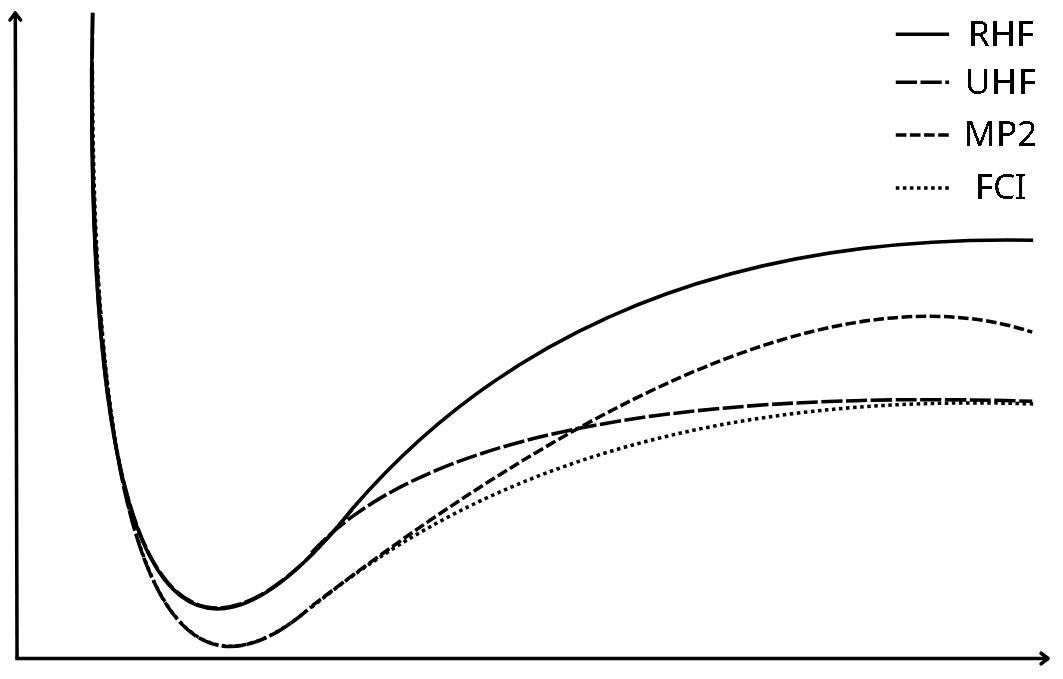
\includegraphics[width=0.8\textwidth]{figures/Ekstra/PES_HF.png} % Replace with actual figure file
    \caption{Potential energy curves for the Hydrogen atom illustrating the failure of HF near dissociation and the importance of electron correlation. The HF curve deviates significantly from the exact FCI curve as the bond is stretched, while MP2 captures much of the correlation energy and follows the FCI curve more closely around the equilibrium bond length. (Adapted from Helgaker et al. \cite{Helgaker2000} Figs. 5.20 and 5.12.)}
    \label{fig:hf_pes}
\end{figure}


\subsection{Møller-Plesset Perturbation Theory}
\label{subsec:mp2}

Møller-Plesset perturbation theory (MPPT) treats electron correlation as a perturbation on top of the mean-field Fock operator. Truncated at second order (MP2), it is the simplest post-HF method that captures dynamical correlation at $\mathcal{O}(O^2V^2)$ computational cost, and furnishes the energy functional that OVOS seeks to optimise.

\subsubsection{MP2 Correlation Energy}

The MP2 correlation energy is derived by partitioning the electronic Hamiltonian as $\hat{H} = \hat{f} + \lambda \hat{V}$, where $\hat{f}$ is the Fock operator, which is diagonal in the canonical molecular orbital basis, and $\hat{V}$ is the fluctuation potential that accounts for electron correlation \cite{Helgaker2000}.
The zeroth-order solution is the Hartree-Fock determinant $|\Phi_0\rangle$. Brillouin's theorem states that singly-excited determinants have zero coupling to $|\Phi_0\rangle$, consequently, first-order perturbation theory contributes no singles terms \cite{Helgaker2000, Jensen2017}. The first-order correction to the wavefunction is therefore a linear combination of doubly-excited determinants only. The associated MP1 amplitudes for these double excitations are:
\begin{align}
    \label{eq:mp1_amps}
    t_{ij}^{ab} = -\frac{\langle ab \| ij \rangle}{\varepsilon_a + \varepsilon_b - \varepsilon_i - \varepsilon_j}
\end{align}

where $\langle ab \| ij \rangle$ is the antisymmetrised two-electron integral in physicists' notation, see Section~\ref{sec:int_notation} for notation details, and the denominator $\varepsilon_a + \varepsilon_b - \varepsilon_i - \varepsilon_j$ is the energy cost of exciting occupied orbitals $i,j$ to virtual orbitals $a,b$. \cite{Helgaker2000, Jensen2017}.

The MP2 correlation energy over all occupied and virtual orbitals is: 
\begin{subequations}
\begin{align}
E_{corr}^{(2)} &= \frac{1}{4} \sum_{i,j,a,b} t_{ij}^{ab} \langle ij \| ab \rangle \label{eq:mp2_full_a} \\
&= \sum_{i>j,a>b} t_{ij}^{ab} \langle ij \| ab \rangle \label{eq:mp2_full_b}
\end{align}
\end{subequations}
where $i,j$ denotes occupied orbitals and virtual orbitals denoted by $a,b$ \cite{Helgaker2000}. In practice, the summation can be restricted to $i > j$ and $a > b$ avoiding double counting, we drop the $1/4$ factor from Equation~\ref{eq:mp2_full_a}, leading to \ref{eq:mp2_full_b}. It is critical to make clear that both of these expressions sum over the entire orbital space the full, occupied and virtual, MP2 energy. In Section~\ref{subsec:2nd_hylleraas}, we will build Equation~\ref{eq:mp2_full_b} with a truncated virtual orbital space, the MP2 energy used in OVOS, reducing computational cost while retaining most correlation energy. In the code implementation in Chapter~\ref{ch:method}, we use the restricted summation convention of Equation~\ref{eq:mp2_full_b} to avoid double counting and ensure consistency with the amplitude definitions. 


\subsubsection{Lower-Order Amplitudes}

In MP2, the MP1 amplitudes correspond to double electron excitations (T2 amplitudes), defined in Equation~\ref{eq:mp1_amps}. The single excitations (S), the T1 amplitudes, do not appear in the MP2 energy expression due to Brillouin's theorem, which states that the matrix elements of the Hamiltonian between the Hartree-Fock determinant and singly-excited determinants vanish \cite{Helgaker2000}. The presence of non-zero T1 amplitudes is an indicator that the reference determinant is not optimal, it suggests that the orbitals can be rotated to lower the energy \cite{Lee2018, Handy1989}.

Including the T2 excitations, T1 and T2 excitations, in addition to the HF state, are commonly referred to as Single-Double (SD) space in regards to methods, e.g. Coupled Cluster SD (CCSD) \cite{Helgaker2000}. Here, the stationarity condition $\nabla_R E(R) = 0$ defines optimal orbitals, which are formalized in quantum chemistry as Brueckner orbitals (named after Brueckner's self-consistency principle) where the T1 amplitudes vanish \cite{Brueckner1954}. This connection between orbital optimization and the nature of the excitation amplitudes is a key motivation for developing methods like OVOS that seek to optimize the virtual orbital space to minimize correlation energy, effectively minimizing the T1 amplitudes \cite{Adamowicz1987}.

\subsubsection{MP2 Limitations and Applicability}

MP2 is size-consistent \cite{Helgaker2000}, meaning that the correlation energy of non-interacting subsystems is additive, see Equation~\ref{eq:mp2_full_b}, which is a crucial property for accurately describing large systems and reaction energies \cite{Jensen2017}. However, MP2 is a single-reference method and can fail in cases where the reference determinant is not a good approximation to the true wavefunction, such as in bond dissociation or transition states  \cite{Helgaker2000, Cao2019}. In such cases, higher-order methods or multi-reference approaches may be necessary to capture the correct physics \cite{Sherrill1999}.

\subsubsection{Computational Scaling Motivation}

The $\mathcal{O}(O^2V^2)$ computational scaling of MP2 presents a significant barrier for large systems and higher-order methods \cite{Jensen2017, Cao2019}. The Optimized Virtual Orbital Space (OVOS) method, detailed in Chapter~\ref{ch:theory}, applies a strategic solution, by restricting the correlation energy calculation to a small, actively-correlated subset of virtual orbitals, the effective scaling can be reduced to $\mathcal{O}(N_{occ}^2 {N'_{virt}}^2)$, where $N'_{virt} \ll N_{virt}$ \cite{Adamowicz1987}. This active space reduction is particularly powerful when combined with higher-order methods like CCSD(T), which scale as $\mathcal{O}(O^3V^4)$ or worse in the full space. For which $V$ reflects the size of the virtual space, and reducing $V$ to $N'_{virt}$ can make previously intractable calculations feasible while retaining much of the correlation energy. This scaling bottleneck directly drives the need for OVOS, especially when aiming for high‑level correlation treatments.


































\section{Background for understanding OVOS}
\label{sec:theory_background_ovos}

This section provides the theoretical background necessary for understanding the Optimized Virtual Orbital Space (OVOS) method developed in this thesis. We will cover the mathematical framework of orbital rotations, the convergence criteria that defines optimal orbitals, and the optimization strategies employed to find these orbitals. This foundation is critical for grasping how OVOS optimizes the virtual orbital space to maximize correlation energy while maintaining computational efficiency. The concepts introduced here will be directly applied in the implementation of OVOS in Chapter~\ref{ch:method}.


\subsection{Orbital Rotations and Stationarity}

Orbital optimization in post-HF methods relies on rotating the molecular orbitals to minimize a target energy functional, such as the MP2 correlation energy in the case of OVOS. Here we set up the rotation formalism and the stationarity condition needed to derive the OVOS equations.


\subsubsection{Partitioning}

Orbitals in electronic structure theory are often partitioned into different subspaces to facilitate the formulation of post-HF methods. The OVOS method partitions the full spin-orbital basis into three non-overlapping subsets, occupied, active unoccupied (active virtual), and inactive unoccupied (inactive virtual), see Figure~\ref{fig:orbital_partitioning}(1). The occupied orbitals, denoted by indices $i, j, k, l$, correspond to the spin-orbitals that are occupied in the HF reference state, and they are indexed from $0$ to $n_{elec}-1$, where $n_{elec}$ is the number of electrons. The active virtual orbitals, denoted by indices $a, b, c, d$, are the subset of unoccupied orbitals that are optimised in the OVOS method, and they are indexed from $n_{elec}$ to $n_{elec} + N'_{virt} - 1$, where $N'_{virt}$ is the number of active virtual orbitals and is a key parameter in the OVOS method. The inactive virtual orbitals, denoted by indices $e, f, g, h$, are the remaining unoccupied orbitals that are not explicitly rotated in the OVOS method. They define the complement space and are indexed from $n_{elec} + N'_{virt}$ to $n_{spin} - 1$, where $n_{spin}$ is the total number of spin-orbitals. The index notation is summarised in Table~\ref{tab:index_notation}. The OVOS rotation operates only in the block that couples the active virtuals with the inactive virtuals while the occupied orbitals remain fixed, see Figure~\ref{fig:orbital_partitioning}(2). The full set of virtual orbitals can be denoted as $a..e$, which includes all orbitals from $n_{elec}$ to $n_{spin}-1$ for a full MP2 calculation, see Figure~\ref{fig:orbital_partitioning}(3).

\begin{figure}[ht]
    \centering
    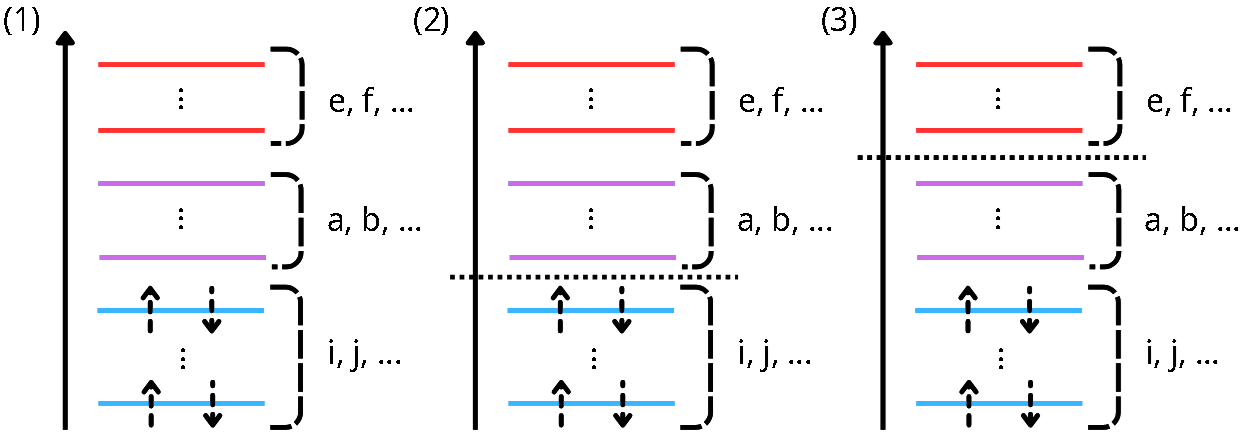
\includegraphics[width=0.8\textwidth]{figures/Ekstra/orbital_partioning.png} % Replace with actual figure file
    \caption{Partitioning of spin-orbital space for OVOS into occupied (blue), active virtual (purple), and inactive virtual subspaces (red). (1) No partitioning. (2) Occupied and unoccupied orbitals. (3) Active and inactive subsets.}
    \label{fig:orbital_partitioning}
\end{figure}

\begin{table}[ht]
    \centering
    \begin{tabular}{|c|c|c|c|c|}
        \hline
        Label & Indices & Orbital Space & Range & Count \\
        \hline
        Occupied & $i,j,k,l$ & occ. & $[0, n_{elec})$ & $n_{elec}$ \\
        Active Virtual & $a,b,c,d$ & act. virt. & $[n_{elec}, n_{elec}+N'_{virt})$ & $N'_{virt}$ \\
        Inactive Virtual & $e,f,g,h$ & inact. virt. & $[n_{elec}+N'_{virt}, n_{spin})$ & $N_{virt}-N'_{virt}$ \\
        All Virtual & $a..h$ & full virt. & $[n_{elec}, n_{spin})$ & $N_{virt}$ \\
        \hline
    \end{tabular}
    \caption{Orbital subspace notation used throughout this thesis.}
    \label{tab:index_notation}
\end{table}

By this partitioning scheme, the OVOS method focuses on optimising the active virtual subspace to minimize the correlation energy, while the inactive virtuals provide a fixed reference that defines the complement space \cite{Adamowicz1987}. This truncation reduces the computational cost of MP2 from $\mathcal{O}(O^2V^2)$ to $\mathcal{O}(O^2N'^2)$, where $N'$ is the number of active virtuals, which is typically much smaller than the total number of virtuals $N'<V$. The choice of $N'$ is a critical aspect of the OVOS method, as it involves a trade-off between accuracy and computational cost.




\subsection{The Second-Order Hylleraas Functional}
\label{subsec:2nd_hylleraas}

OVOS minimises the second-order Hylleraas functional $J_2$ with respect to the choice of active virtual orbitals \cite{Adamowicz1987}. This section seeks to derive $J_2$ from the second-order Rayleigh-Schrödinger perturbation expression and to establish its connection to the MP2 correlation energy.

\subsubsection{From Perturbation Theory to the Hylleraas Principle}
We arrive at the Hylleraas functional by starting from the Rayleigh-Schrödinger (RS) perturbation theory expression for the second-order energy correction \cite{Helgaker2000}, starting by an expansion of the total energy:
\begin{equation}
E = E^{(0)} + E^{(1)} + E^{(2)} + \ldots
\end{equation}
where the zeroth-order energy $E^{(0)}$ is the energy of the zero-order Hamiltonian $H_0$ (The Fock Operator), and the first-order energy $E^{(1)}$ is the expectation value of the correlation perturbation operator $V = H - H_0$ with respect to the zero-order wavefunction $\Psi^{(0)}$,
\begin{equation}
    E^{(1)} = \langle\Psi^{(0)}|V|\Psi^{(0)}\rangle
\end{equation}
The sum of zero-order and first-order energies, $E^{(0)} + E^{(1)}$, is the Hartree-Fock energy. 

The second-order energy correction $E^{(2)}$ is the MP2 correlation energy, expressed in terms of the correlation perturbation operator $V = H - H_0$ and the first-order wavefunction $\Psi^{(1)}$ as:
\begin{equation}
E^{(2)} = \langle\Psi^{(0)}|V|\Psi^{(1)}\rangle
\end{equation}
where $\Psi^{(0)}$ is the Hartree-Fock reference wavefunction. Using intermediate normalization, $\langle\Psi^{(0)}|\Psi^{(1)}\rangle = 0$, and the first-order Schrödinger equation:
\begin{equation}
    H_0 |\Psi^{(1)}\rangle + V|\Psi^{(0)}\rangle = E^{(0)}|\Psi^{(1)}\rangle + E^{(1)}|\Psi^{(0)}\rangle
\end{equation}
we can rearrange to express:
\begin{equation}
    (H_0 - E^{(0)})|\Psi^{(1)}\rangle = -(V - E^{(1)})|\Psi^{(0)}\rangle
\end{equation}
take the inner product with $\langle\Psi^{(1)}|$:
\begin{equation}
    \langle\Psi^{(1)}|H_0 - E^{(0)}|\Psi^{(1)}\rangle = -\langle\Psi^{(1)}|V - E^{(1)}|\Psi^{(0)}\rangle
\end{equation}
using, $\langle\Psi^{(1)}|E^{(1)}|\Psi^{(0)}\rangle = E^{(1)}\langle\Psi^{(1)}|\Psi^{(0)}\rangle = 0$, we can rewrite the second-order energy correction as:
\begin{equation}
    E^{(2)} \leq \langle\Psi^{(1)}|H_0 - E^{(0)}|\Psi^{(1)}\rangle + 2\langle\Psi^{(1)}|V - E^{(1)}|\Psi^{(0)}\rangle
\end{equation}

The second-order Hylleraas functional $J_2$ is defined as the upper bound to the second-order energy correction, such that $E^{(2)} \leq J_2$ for any choice of $\Psi^{(1)}$. In other words, minimising $J_2$ with respect to $\Psi^{(1)}$ recovers the MP2 correlation energy, $E^{(2)} = \min_{\Psi^{(1)}} J_2$. Minimising by varying $\Psi^{(1)}$ leads to the stationary condition that $\Psi^{(1)}$ must satisfy the first-order Schrödinger equation,
\begin{equation}
    \frac{\partial J_2}{\partial \Psi^{(1)}} = 2 (H_0 - E^{(0)})|\Psi^{(1)}\rangle + 2(V - E^{(1)})|\Psi^{(0)}\rangle = 0
\end{equation}
making the ansatz that $\Psi^{(1)}$ is a linear combination of doubly-excited determinants, $\Psi^{(1)} = \sum_{i>j,a>b} t_{ij}^{ab} |\Phi_{ij}^{ab}\rangle$, and $\Psi^{(0)}$ is the HF reference determinant. We can write out the MP2 amplitudes $t_{ij}^{ab}$ as:
\begin{equation}
    t_{ij}^{ab} = \frac{\langle ij\|ab\rangle}{\epsilon_i + \epsilon_j - \epsilon_a - \epsilon_b}
\end{equation}
where $\langle ij\|ab\rangle$ are the antisymmetrised two-electron integrals in physicists' notation, and $\epsilon_p$ are the orbital energies. 

\subsubsection{Pair Decomposition and Explicit Form of \texorpdfstring{$J_2$}{J2}}
To apply the Hylleraas functional to orbital optimisation, we decompose $J_2$ into unique pairs of occupied orbital indices $i>j$, each pair involves orthogonal configurations, $\langle\Phi_{ij}^{ab}|\Phi_{kl}^{cd}\rangle = 0$ for $(i,j) \neq (k,l)$, which translate to the functional being additively separable, $J_2 = \sum_{i>j} J_{ij}^{(2)}$, each pair contributes:
\begin{equation}
    J_{ij}^{(2)} = \langle\Psi^{(1)}_{ij}|H_0 - E^{(0)}|\Psi^{(1)}_{ij}\rangle + 2\langle\Psi^{(1)}_{ij}|V - E^{(1)}|\Psi^{(0)}\rangle
\end{equation}
where we moved the sum over $i>j$ inside the definition of $\Psi^{(1)}_{ij}$ out to allow writing the decomposed form. Futhermore, we can decompose $J_{ij}^{(2)}$ into two contributions, the expectation value of the zero-order Hamiltonian (first term) and the coupling to the reference state via the perturbation operator (second term). 

\subsubsection{The Zero-Order Term}
The "diagonal" term takes the form when we evaluate the expectation value:
\begin{equation}
    \langle\Psi^{(1)}_{ij}|H_0 - E^{(0)}|\Psi^{(1)}_{ij}\rangle = \sum_{a>b,c>d} t_{ij}^{ab} t_{ij}^{cd} \langle\Phi_{ij}^{ab}|(H_0 - E^{(0)})|\Phi_{ij}^{cd}\rangle
\end{equation}
To evaluate, we recall that $H_0 = \sum_i f_{ii}$, where $f_{pq}$ is the Fock matrix element. The first-order energy is $E^{(0)} = \sum_i \epsilon_i$, which represents the sum of occupied orbital energies. The matrix element of $H_0$ between the doubly-excited determinants can be evaluated to:
\begin{equation}
    \langle\Phi_{ij}^{ab}|H_0|\Phi_{ij}^{cd}\rangle = f_{ac}\delta_{bd} - f_{ad}\delta_{bc} + f_{bd}\delta_{ac} - f_{bc}\delta_{ad}
\end{equation}
The four term Fock structure arises from the antisymmetrised electron exchange and orbital index rearrangements, $\langle\Phi_{ij}^{ab}|f_{pq}|\Phi_{ij}^{cd}\rangle$ is non-zero only when the orbital indices match, which is selected by the $\delta$ structure.

The matrix element of $E^{(0)}$ is:
\begin{equation}
    \langle\Phi_{ij}^{ab}|E^{(0)}|\Phi_{ij}^{cd}\rangle = (\epsilon_i + \epsilon_j)(\delta_{ac}\delta_{bd} - \delta_{ad}\delta_{bc})   
\end{equation}
Combined, the "diagonal" term becomes:
\begin{align}
    \langle\Psi^{(1)}_{ij}|H_0 - E^{(0)}|\Psi^{(1)}_{ij}\rangle &= \sum_{a>b,c>d} t_{ij}^{ab} t_{ij}^{cd} [ (f_{ac}\delta_{bd} - f_{ad}\delta_{bc} + f_{bd}\delta_{ac} - f_{bc}\delta_{ad}) \\ &\qquad \qquad - (\epsilon_i + \epsilon_j)(\delta_{ac}\delta_{bd} - \delta_{ad}\delta_{bc}) ]
\end{align}


\subsubsection{Evaluation of the Perturbative Coupling}
The "off-diagonal" term, consisting of the perturbation operator $V$ and the first-order energy $E^{(1)}$, assesses the coupling between the reference determinant and the doubly-excited determinants. Evaluating the matrix element gives for each:
\begin{equation}
    \langle\Psi^{(1)}_{ij}|V|\Psi^{(0)}\rangle = \sum_{a>b} t_{ij}^{ab} \langle ij\|ab\rangle
\end{equation}
and,
\begin{equation}
    \langle\Psi^{(1)}_{ij}|E^{(1)}|\Psi^{(0)}\rangle = E^{(1)} \langle\Psi^{(1)}_{ij}|\Psi^{(0)}\rangle = 0
\end{equation}
therefore the "off-diagonal" term reduces to:
\begin{equation}
    2\langle\Psi^{(1)}_{ij}|V - E^{(1)}|\Psi^{(0)}\rangle = 2\sum_{a>b} t_{ij}^{ab} \langle ij\|ab\rangle
\end{equation}

The final expression for $J_{ij}^{(2)}$ is then:
\begin{equation}
    J_{ij}^{(2)} = \sum_{a>b,c>d} t_{ij}^{ab} t_{ij}^{cd} (f_{ac}\delta_{bd} - f_{ad}\delta_{bc} + f_{bd}\delta_{ac} - f_{bc}\delta_{ad} - (\epsilon_i + \epsilon_j)(\delta_{ac}\delta_{bd} - \delta_{ad}\delta_{bc})) + 2\sum_{a>b} t_{ij}^{ab} \langle ij\|ab\rangle
\end{equation}


As such we derived the explicit form of the second-order Hylleraas functional $J_2$ in terms of the MP2 amplitudes $t_{ij}^{ab}$, the Fock matrix elements $f_{pq}$, and the antisymmetrised two-electron integrals $\langle ij\|ab\rangle$. This functional serves as the target for orbital optimization in OVOS, where the active virtual orbitals are rotated to minimize $J_2$.


\subsection{Orbital Rotation Parameterisation}

Optimising orbitals in OVOS is achieved by applying a unitary transformation, rotating the virtual orbitals to maximise the correlation energy captured by the active space \cite{Adamowicz1987}. This section introduces the mathematical formalism of orbital rotations, parameterised by an antisymmetric matrix $\mathbf{R}$, and how the unitary transformation $\mathbf{U} = e^{\mathbf{R}}$ is constructed to mix only the active and inactive virtual orbitals.


\subsubsection{Orbital Rotation}

Orbital rotations can be represented mathematically as unitary transformations of the molecular orbital coefficients \cite{Helgaker2000}. A unitary transformation can be expressed as $U = e^R$, where $R$ is an antisymmetric matrix that parameterizes the rotation. The new orbital coefficients after rotation are given by $C_{new} = C_{old} U$. The effect of this rotation on the one-electron integrals is given by $h_{new} = U^\dagger h_{old} U$, and for the two-electron integrals, the transformation is more complex due to their four-index nature, but it can be expressed as $g_{new} = U^\dagger g_{old} U$ in a suitable tensor contraction form. The Fock matrix also transforms under the same unitary rotation: $F_{new} = U^\dagger F_{old} U$. The use of unitary transformations ensures that the orthonormality of the orbitals is preserved during the optimization process \cite{Helgaker2000}. 

\subsubsection{Active and Inactive Virtual Subspaces}

The antisymmetric matrix $\mathbf{R}$ is defined such that only the block corresponding to active-inactive virtual orbital mixing is non-zero. Specifically, $R_{ae}$ is non-zero, while all other blocks (e.g., occupied-occupied $R_{ij}$, active-active $R_{ab}$, inactive-inactive $R_{ef}$) are zero.

We can restrict the orbital rotations to only mix active and inactive virtual orbitals because active-active rotations do not change the value of $J_2$, as $J_2$ depends only on the choice of optimised orbitals and not on their specific linear combinations of basis states. In other words, any rotation within the active space leaves $J_2$ invariant:
\begin{equation}
    J_2[\{\phi_a\}] = J_2[\{\sum_b U_{ab}\phi_b\}]
\end{equation}
Inactive-inactive rotations do not affect the active space at all. We neglect all mixing with and between occupied orbitals, as it is not within the scope of the OVOS method.

We can write the full matrix $\mathbf{R}$ as:
\begin{equation}
    R = 
    \begin{bmatrix}
        R_{ij} & R_{ia} & R_{ie} \\
        R_{aj} & R_{ab} & R_{ae} \\
        R_{ej} & R_{eb} & R_{ef}
    \end{bmatrix}
    = 
    \begin{bmatrix}
        0 & 0 & 0 \\
        0 & 0 & R_{ae} \\
        0 & -R_{ae}^T & 0
    \end{bmatrix}
\end{equation}
where we relate the active-inactive block to its transpose by the antisymmetry condition, $R_{ea} = -R_{ae}$. The dimension of the non-zero block is $N' \times (N_{\rm unocc.} - N')$.

\subsubsection{Unitary Transformation via Matrix Exponential}

The unitary transformation $\mathbf{U}$ that rotates the orbitals is given by the matrix exponential of $\mathbf{R}$:
\begin{equation}
    \mathbf{U} = e^{\mathbf{R}} = \sum_{n=0}^{\infty} \frac{\mathbf{R}^n}{n!}
\end{equation}
Unitary by construction, $\mathbf{U}^\dagger \mathbf{U} = \mathbf{I}$, is guaranteed by the antisymmetry of $\mathbf{R}$, $R = -R^\dagger$. 

Expanding the virtual orbitals to second order in $\mathbf{R}$ gives:
\begin{equation}
    \phi'_a = \sum_b U_{ab} \phi_b + \sum_e U_{ae} \phi_e
\end{equation}
We can express an active orbital after rotation as:
\begin{equation}
    \phi'_a = \phi_a + \sum_e R_{ea}\phi_e - \frac{1}{2}\sum_{b,e} R_{ea}R_{eb}\phi_b + \ldots
\end{equation}
where the original active orbital is mixed with the inactive orbitals via the first-order term, and the second-order term accounts for the fact that the new active orbital is no longer orthogonal to the original active orbitals. These terms are redundant when applying the full matrix exponential instead, as it handles all terms, the expansion allows for a tractable expression for the gradient and Hessian of $J_2$ with respect to the rotation parameters, which are derived in the following sections.



\subsection{Gradient Expression}

The descent direction for OVOS optimisation is given by the gradient of the Hylleraas functional $J_2$ with respect to the orbital rotation parameters $R_{ae}$ \cite{Adamowicz1987}. This section derives the expression for the gradient, which consists of two terms, a direct contribution from the active-inactive mixing and an indirect contribution via the MP2 virtual-virtual density matrix $D_{ab}$.


\subsubsection{MP2 Virtual-Virtual Density Matrix}

The second-order density matrix, which captures the correlation between pairs of active virtual orbitals, how strongly active virtual orbitals, how strongly $a$ and $b$ appear together in the MP1 wavefunction, is defined as:
\begin{equation}
    D_{ab} = \sum_{i>j}\sum_c t_{ij}^{ac} t_{ij}^{bc}
\end{equation}
where $t_{ij}^{ac}$ are the MP2 amplitudes. The matrix $D_{ab}$ is symmetric, $D_{ab} = D_{ba}$, 

\subsubsection{Gradient Expression}
\label{subsubsec:gradient}

The gradient of $J_2$ with respect to the orbital rotation parameters $R_{ae}$ is given by:
\begin{equation}
    G_{ae} = \frac{\partial J_2}{\partial R_{ae}} \bigg|_{R=0} 
\end{equation}
Here we evaluate the gradient at $R=0$ to obtain the expression in terms of the unrotated orbitals. This condition means the Fock matrix and integrals are evaluated in the original orbital basis, such that the orbitals are canonical in the unoccupied space. This means in the Hylleraas functional, the Fock matrix elements $f_{ac}$ are diagonal in the virtual space, $f_{ac} = \epsilon_a \delta_{ac}$, meaning we can express the "zero-order" term of $J_2$ in terms of the orbital energies:
\begin{align}
    \langle\Psi^{(1)}_{ij}|H_0 - E^{(0)}|\Psi^{(1)}_{ij}\rangle 
    &= \sum_{a>b,c>d} t_{ij}^{ab} t_{ij}^{cd} [ (\epsilon_a \delta_{ac}\delta_{bd} - \epsilon_a \delta_{ad}\delta_{bc} + \epsilon_b \delta_{bd}\delta_{ac} - \epsilon_b \delta_{bc}\delta_{ad}) \\ &\qquad \qquad - (\epsilon_i + \epsilon_j)(\delta_{ac}\delta_{bd} - \delta_{ad}\delta_{bc})] \\
    &= \sum_{a>b,c>d} t_{ij}^{ab} t_{ij}^{cd} [ (\epsilon_a + \epsilon_b - \epsilon_i - \epsilon_j)(\delta_{ac}\delta_{bd} - \delta_{ad}\delta_{bc}) ]
\end{align}
using the definition of the MP2 amplitudes, we can express the "zero-order" term as:
\begin{align}
    \langle\Psi^{(1)}_{ij}|H_0 - E^{(0)}|\Psi^{(1)}_{ij}\rangle 
    &= - \sum_{a>b,c>d} t_{ij}^{cd}  \langle ij\|ab\rangle (\delta_{ac}\delta_{bd} - \delta_{ad}\delta_{bc}) \\
    &= - \sum_{a>b} t_{ij}^{ab} \langle ij\|ab\rangle
\end{align}
as only the first deltas term contributes, by the summation convention. Recognize the resulting expression as the "perturbative coupling" term, therefore the $J_2$ functional can be expressed as:
\begin{equation}
    J_2 = \sum_{i>j}\sum_{a>b} t_{ij}^{ab} \langle ij\|ab\rangle = \sum_{i>j}\sum_{a>b} \langle ij\|ab\rangle \langle ij\|ab\rangle / (\epsilon_i + \epsilon_j - \epsilon_a - \epsilon_b)
\end{equation}

Using the chain rule to evaluate the gradient, in regards to the two-electron integrals and the Fock matrix elements, we get the intermediate expression:
\begin{align}
    \frac{\partial J_2}{\partial R_{ae}} 
    &=
    \sum_{i>j}\sum_{a>b} 2 \langle ij\|ab\rangle / (\epsilon_i + \epsilon_j - \epsilon_a - \epsilon_b) \frac{\partial \langle ij\|ab\rangle}{\partial R_{ae}}
    \\
    &- \sum_{i>j}\sum_{a>b} (\langle ij\|ab\rangle / (\epsilon_i + \epsilon_j - \epsilon_a - \epsilon_b))^2 \frac{\partial}{\partial R_{ae}} (\epsilon_i + \epsilon_j - \epsilon_a - \epsilon_b)
\end{align}
here each term is evaluated to:
\begin{equation}
    \frac{\partial \langle ij\|ab\rangle}{\partial R_{ae}} = \langle ij\|eb\rangle
    \quad \text{and} \quad
    \frac{\partial}{\partial R_{ae}} (\epsilon_i + \epsilon_j - \epsilon_a - \epsilon_b) = - f_{ea} 
\end{equation}
arriving at the final expression for the gradient:
\begin{align}
    G_{ae} = \frac{\partial J_2}{\partial R_{ae}} 
    &= 2\sum_{i>j}\sum_{b} t_{ij}^{ab} \langle ij\|eb\rangle + 2 \sum_{b} D_{ab} f_{eb}
\end{align}
where we have substituted the definition of the density matrix $D_{ab}$ and renamed the indices for clarity. The first term captures the direct contribution of the active-inactive mixing to $J_2$, while the second term captures the contribution via the density matrix, which accounts for how optimised orbitals are correlated with each other in the MP1 wavefunction. At convergence, the gradient must vanish, $G_{ae} = 0$ for all $a,e$, a stationarity condition that defines the optimal orbitals. The gradient is a matrix of dimension $(N_{\rm virt} - N') \times N'$. 


\subsubsection{The Stationarity Principle}

 Optimal orbitals are referred by the stationarity condition that the gradient goes to zero: $\nabla_R E(R) \rightarrow 0$. This condition implies that the energy is at a local extremum with respect to orbital rotations. The stationary point can correspond to a local minimum, maximum, or saddle point in the energy landscape, by examining the second derivative (Hessian) at the stationary point, we can determine the nature of the extremum. For this purpose we derive the Hessian matrix in the following. % The connection between this stationarity principle and specific types of optimal orbitals, such as OO-MP2 and Brueckner orbitals, arises from the particular form of the energy functional being optimized \cite{Lee2018, Handy1989}. 


\subsection{Hessian Expression}

Taking the second derivative of the Hylleraas functional with respect to the orbital rotation parameters $R_{ae}$ and $R_{fb}$, we arrive at the Hessian matrix:
\begin{align}
    H_{ae,bf} &= \frac{\partial^2 J_2}{\partial R_{ae} \partial R_{bf}} \bigg|_{R=0}
\end{align}
If the gradient captures the slope of the energy landscape, the Hessian captures the curvature, providing information about how the energy changes as we move in different directions in orbital space.

Adamowicz and Bartlett derive the full expression for the Hessian, which consists of four terms:
\begin{align}
    H_{ae,bf} &= 2\sum_{i>j} t_{ij}^{ab}\langle ij\|ef\rangle
               - \sum_{i>j}\sum_c [t_{ij}^{ac}\langle ij\|bc\rangle
               + t_{ij}^{bc}\langle ij\|ca\rangle] \delta_{ef}
               \\ &\qquad + D_{ab}(f_{aa} - f_{bb}) \delta_{ef}
               + D_{ab} f_{ef}(1-\delta_{ef})
\end{align}
they note the active orbitals are canonical, and that the Hessian also shows pair separability  \cite{Adamowicz1987}. 

\subsubsection{Derivation of the Hessian Expression}

We start from the MP2 gradient written with consistent dummy indices:
\begin{equation}
    G_{ae} = 2\sum_{i>j}\sum_c t_{ij}^{ac}\langle ij||ec\rangle + 2\sum_c D_{ac}f_{ec}
\end{equation}
where
\begin{equation}
    D_{ac} = \sum_{i>j}\sum_d t_{ij}^{ad}t_{ij}^{cd}, 
    \qquad 
    f_{ec} = \epsilon_e \delta_{ec}
\end{equation}

The Hessian is defined as:
\begin{equation}
    H_{ea,fb} = \frac{\partial G_{ae}}{\partial R_{bf}}
\end{equation}

We use the following standard orbital-rotation derivatives.

\paragraph{Two-electron integrals:}
\begin{equation}
\frac{\partial \langle ij||ec\rangle}{\partial R_{bf}} =
\delta_{cb}\langle ij||ef\rangle
+ \delta_{eb}\langle ij||fc\rangle
- \delta_{cf}\langle ij||eb\rangle
- \delta_{ef}\langle ij||bc\rangle
\end{equation}

\paragraph{Fock matrix (canonical orbitals):}
\begin{equation}
\frac{\partial f_{ec}}{\partial R_{bf}} =
\delta_{cb}f_{ef}
+ \delta_{eb}f_{fc}
- \delta_{cf}f_{eb}
- \delta_{ef}f_{bc}
\end{equation}

\paragraph{Amplitudes:}

Rather than expanding the full quotient rule, we use:
\begin{equation}
t_{ij}^{ac} = \frac{\langle ij||ac\rangle}{\Delta_{ijac}}
\end{equation}
and differentiate formally, allowing cancellation later:
\begin{equation}
\frac{\partial t_{ij}^{ac}}{\partial R_{bf}} =
\frac{1}{\Delta_{ijac}} \frac{\partial \langle ij||ac\rangle}{\partial R_{bf}}
- t_{ij}^{ac} \frac{1}{\Delta_{ijac}} \frac{\partial \Delta_{ijac}}{\partial R_{bf}}
\end{equation}

\subsubsection{Step 1: Differentiate First Gradient Term}

Define:
\begin{equation}
A = \frac{\partial}{\partial R_{bf}}
\left(2\sum_{i>j}\sum_c t_{ij}^{ac}\langle ij||ec\rangle\right)
\end{equation}

Apply product rule:
\begin{align}
A &= 2\sum_{i>j}\sum_c
\left(
\frac{\partial t_{ij}^{ac}}{\partial R_{bf}}\langle ij||ec\rangle
+
t_{ij}^{ac}\frac{\partial \langle ij||ec\rangle}{\partial R_{bf}}
\right)
\end{align}

\textbf{Integral derivative contribution}

Insert the integral derivative:
\begin{align}
\sum_c t_{ij}^{ac}\frac{\partial \langle ij||ec\rangle}{\partial R_{bf}}
&=
\sum_c t_{ij}^{ac}
\left(
\delta_{cb}\langle ij||ef\rangle
+ \delta_{eb}\langle ij||fc\rangle
- \delta_{cf}\langle ij||eb\rangle
- \delta_{ef}\langle ij||bc\rangle
\right)
\end{align}

Collapse sums:
\begin{align}
&= t_{ij}^{ab}\langle ij||ef\rangle
+ \delta_{eb}\sum_c t_{ij}^{ac}\langle ij||fc\rangle
- t_{ij}^{af}\langle ij||eb\rangle
- \delta_{ef}\sum_c t_{ij}^{ac}\langle ij||bc\rangle
\end{align}

Thus:
\begin{align}
A_{\text{int}} =
2\sum_{i>j}
\Big[
t_{ij}^{ab}\langle ij||ef\rangle
- t_{ij}^{af}\langle ij||eb\rangle
\Big]
+ 2\delta_{eb}\sum_{i>j}\sum_c t_{ij}^{ac}\langle ij||fc\rangle
- 2\delta_{ef}\sum_{i>j}\sum_c t_{ij}^{ac}\langle ij||bc\rangle
\end{align}

\textbf{Amplitude derivative contribution}

The amplitude derivative produces terms of the same structure but with permuted indices. After relabeling dummy indices and combining symmetric contributions, these terms cancel the $\delta_{eb}$ terms and generate the symmetric partner of the $\delta_{ef}$ term:
\begin{equation}
- 2\delta_{ef}\sum_{i>j}\sum_c t_{ij}^{bc}\langle ij||ca\rangle
\end{equation}

\textbf{Final result for A}

\begin{align}
A =
2\sum_{i>j} t_{ij}^{ab}\langle ij||ef\rangle
- \delta_{ef}\sum_{i>j}\sum_c
\left[
t_{ij}^{ac}\langle ij||bc\rangle
+
t_{ij}^{bc}\langle ij||ca\rangle
\right]
\end{align}

\subsubsection{Step 2: Differentiate Second Gradient Term}

Define:
\begin{equation}
B = \frac{\partial}{\partial R_{bf}}\left(2\sum_c D_{ac}f_{ec}\right)
\end{equation}

\begin{align}
B = 2\sum_c
\left(
\frac{\partial D_{ac}}{\partial R_{bf}}f_{ec}
+
D_{ac}\frac{\partial f_{ec}}{\partial R_{bf}}
\right)
\end{align}

\textbf{Fock derivative term}

\begin{align}
\sum_c D_{ac}\frac{\partial f_{ec}}{\partial R_{bf}}
&=
\sum_c D_{ac}
\left(
\delta_{cb}f_{ef}
- \delta_{ef}f_{bc}
\right)
\\
&=
D_{ab}f_{ef}
- \delta_{ef}\sum_c D_{ac}f_{bc}
\end{align}

\textbf{Density derivative term}

After inserting amplitude derivatives and simplifying (using symmetry and relabeling), this yields:
\begin{equation}
\delta_{ef} D_{ab}(f_{aa} - f_{bb})
\end{equation}

\textbf{Final result for B}

\begin{equation}
B =
D_{ab}(f_{aa}-f_{bb})\delta_{ef}
+ D_{ab} f_{ef}(1-\delta_{ef})
\end{equation}

\subsubsection{Final Hessian}

\begin{align}
H_{ea,fb} &=
2\sum_{i>j} t_{ij}^{ab}\langle ij||ef\rangle
\\
&\quad
- \delta_{ef}\sum_{i>j}\sum_c
\left[
t_{ij}^{ac}\langle ij||bc\rangle
+
t_{ij}^{bc}\langle ij||ca\rangle
\right]
\\
&\quad
+ D_{ab}(f_{aa}-f_{bb})\delta_{ef}
+ D_{ab} f_{ef}(1-\delta_{ef})
\end{align}


\subsubsection{Block Structure of the Hessian}

We see a clear simplification of the Hessian if $\delta_{ef}=0$:
\begin{align}
    H_{ae,bf} &= 2\sum_{i>j} t_{ij}^{ab}\langle ij\|ef\rangle
               + D_{ab} f_{ef}
\end{align}
such that two orbitals $a,b$ would not rotate to the same orbitals, on the other hand if $\delta_{ef}=1$:
\begin{align}
    H_{ae,be} &= 2\sum_{i>j} t_{ij}^{ab}\langle ij\|ee\rangle
               - \sum_{i>j}\sum_c [t_{ij}^{ac}\langle ij\|bc\rangle
               + t_{ij}^{bc}\langle ij\|ca\rangle]
               + D_{ab}(f_{aa} - f_{bb})
\end{align}
such that two orbitals $a,b$ would rotate to the same orbital. This translates to a block structure within the Hessian, where each block corresponds to a specific inactive orbital $e$. Each block is a square matrix of size $N' \times N'$, where $N'$ is the number of optimised orbitals. The off-diagonal blocks (where $e \neq f$) contain terms that couple different inactive orbitals, but these are typically smaller in magnitude than the diagonal blocks. This block structure approximation allows for efficient inversion of the Hessian, as each block can be inverted separately, reducing the computational cost from inverting a large matrix to inverting several smaller matrices.

\subsubsection{Negative Eigenvalues and Level-Shift Stabilisation}

As the Hessian expresses the curvature of the energy landscape, it may become indefinite (i.e., have negative eigenvalues) near saddle points or in cases with small virtual orbital energy gaps. This can lead to divergence or oscillations in the Newton-Raphson optimization, see next section. To address this, a level-shift strategy can be employed, if any diagonal block of the Hessian has negative eigenvalues, a positive shift $\lambda$ is added to the diagonal elements, effectively replacing $\mathbf{H}$ with $\mathbf{H} + \lambda\mathbf{I}$. The choice of $\lambda$ can be empirical or based on a dynamic threshold related to the smallest eigenvalue. This ensures that the modified Hessian is positive-definite, allowing for stable convergence towards a local minimum. Adamowicz \& Bartlett does not discuss this strategy. It is observed that the block approximation does get rid of most negative eigenvalues, but some may still remain, which may be in cases with small virtual gaps $\epsilon_a - \epsilon_i$ from basis sets with diffuse functions. The implementation of OVOS omits the level-shift strategy, but it is a potential avenue for future improvement to ensure robust convergence.



\subsection{Newton-Raphson}

Building off the gradient and Hessian of $J_2$, an orbital rotation update $\Delta\mathbf{R}$ can be computed using the Newton-Raphson (NR) method, which iteratively refines the orbital coefficients to minimize $J_2$. The NR update is given by:
\begin{equation}
    \mathbf{R} = - \mathbf{G} \cdot \mathbf{H}^{-1}
\end{equation}
which is equivalent to:
\begin{equation}
    \mathbf{H} \mathbf{R} = - \mathbf{G}
\end{equation}
where $\mathbf{G}$ is the gradient vector and $\mathbf{H}$ is the Hessian matrix. The NR method runs into problems if the energy landscape is flat or has multiple minima, convergence can be slow or may require damping of the update step. The block-diagonal structure of the Hessian allows for efficient inversion, as each block can be treated independently, which is equivalent to solving a reduced linear equation in each inactive-orbital block. To ensure numerical stability, especially in cases where the Hessian may have negative eigenvalues, a level-shift strategy can be applied, as discussed in the previous section. 

The convergence criterion for the NR iterations is typically defined as $|J_2{(n)} - J_2{(n-1)}| < 10^{-8}$, indicating that the change in the Hylleraas functional between iterations is sufficiently small to consider the solution converged. Supplementing this with the stationarity condition $\nabla_R E(R) < 10^{-8}$ ensures that the orbitals are at a local extremum of the energy landscape, which is the defining characteristic of optimal orbitals in this context.  




\subsection{Orbital Canonicalisation}

After a unitary rotation, the virtual Fock block $F_{ab}^{\rm active}$ is generally non-diagonal, meaning the active virtual orbitals are no longer canonical \cite{Helgaker2000}. To restore the canonical form, we compute the active Fock block in the rotated basis:
\begin{equation}
    F_{ab} = \mathbf{C'}^\dagger\, F^{\rm AO}\, \mathbf{C'}
\end{equation}
where $\mathbf{C'}$ are the coefficients of the virtual orbitals after rotation. Diagonalising $F_{ab}$ yields new canonical virtual orbitals with well-defined orbital energies $\varepsilon_a$ from the eigenvalues. This step is crucial for the next iteration of MP2 amplitude calculations, as it ensures that the denominators in the amplitude expressions are based on canonical orbital energies, simplifying the computations and improving numerical stability. It is important to note that only the virtual orbitals are rotated and re-canonicalised at each OVOS iteration; the occupied orbitals remain unchanged throughout the procedure.

With canonical rotated orbitals, the MP2 energy for the new active space can be evaluated, and the energy recovery fraction can be defined to quantify the performance of the OVOS procedure. 

\subsection{Computational Cost and Scaling}
\label{subsec:scaling}

A central motivation for OVOS is the potential for significant computational speedup by contracting the orbital space to a smaller active orbital set \cite{Adamowicz1987}. To quantify this, we analyse the computational cost of each step in the OVOS iteration and compare it to the cost of traditional full-space correlation methods.

\subsubsection{Per-Iteration Cost of OVOS Optimisation}

Defining the cost of an action requires introducing the Big O notation, which describes the asymptotic scaling of an algorithm with respect to the size of the input. In the context of OVOS, the relevant input sizes are the number of occupied orbitals ($N_{occ}$), the number of inactive virtual orbitals ($N_{inact}$), the number of optimized orbitals ($N'$), and the number of atomic orbitals ($n$).

The computational cost of one OVOS iteration can be broken down by the steps involved, see Section 4.1 for an algorithm summary, where the cost are:
\begin{itemize}
    \item Integral transformation: $O(n^4 + N_{occ}^2 N_{virt}^2)$ for transforming two-electron integrals to the MO basis.
    \item MP2 amplitude evaluation: $O(N_{occ}^2 N'^2)$ for computing the amplitudes in the active space.
    \item MP2 energy: $O(N_{occ}^2 N'^4)$ for evaluating the MP2 energy with the active space amplitudes.
    \item Density matrix $D_{ab}$: $O(N_{occ}^2 N'^3)$ for computing the virtual-virtual density matrix.
    \item Gradient $G_{ea}$: $O(N_{occ}^2 N' N_{inact})$ for computing the gradient with respect to orbital rotations.
    \item Hessian $H_{ea,fb}$: $O(N_{occ}^2 N_{inact}^2 N'^2)$ for computing the Hessian in block-diagonal form.
    \item Block diagonal: $O(N_{inact} N'^2)$ for extracting the block-diagonal part of the Hessian.
    \item Newton-Raphson step: $O(N_{inact} N'^3)$ inverting the block-diagonal Hessian.
    \item Orbital rotation: $O((N_{occ}+ N_{inact} + N')^3)$ for computing the unitary rotation matrix via matrix exponential.
    \item Canonicalisation: $O(N'^3)$ for diagonalising the active Fock block to obtain canonical orbitals.
\end{itemize}
Overall, the per-iteration cost is dominated differently for a few cases, summarized in the following table:
\begin{table}[h]
    \centering
    \small
    \begin{tabular}{c|c|c|c|c}
        \textbf{Active Space} & \textbf{$r = N'/N_{\text{virt}}$} & \textbf{Dominant} & \textbf{Cost Scaling} & \textbf{Relative Cost} \\
        \hline
        \textbf{Small} & $\sim 0.1$ & Orbital Rotation & $O(N_{\text{total}}^3)$ & Fastest, but minimal speedup \\
        \textbf{Medium} & $\sim 0.3$–$0.5$ & Newton Solver* & $O((N_{\text{inact}} N')^3)$ & \textbf{Optimal window} \\
        \textbf{Large} & $\sim 0.7$–$0.9$ & MP2 Energy & $O(N_{\text{occ}}^2 N'^4)$ & Diminishing returns \\
        \hline
    \end{tabular}
    \caption{Dominant computational steps in OVOS iterations as a function of the active space size $N'$. *MP2 close 2nd.}
\end{table}
This reflects the trade-off in OVOS, a smaller active spaces reduce the cost of MP2 energy and gradient evaluations but increase the relative cost of orbital rotations and Hessian inversions (number of blocks). Larger active spaces reduce the cost of orbital rotations but increase the cost of MP2 energy evaluations. The optimal window for OVOS is typically in the medium range, where the cost of the Newton step is manageable and the speedup from reduced MP2 evaluations is significant.

Taken the size of the basis set into account, translating to the number of virtual orbitals, the per-iteration cost of OVOS is dominated by the MP2 energy evaluation step, which scales as $O(N_{occ}^2 N'^4)$. However, since $N' < N_{virt}$, this represents a significant reduction compared to the full-space MP2 cost as the basis set size increases, beating out the cost of orbital rotations and Hessian inversions.

\subsubsection{Comparison: Full Virtual Space vs OVOS-Reduced}

In a traditional full-space MP2 calculation, the cost scales as $O(N_{occ}^2 N_{virt}^4)$ due to the need to consider all virtual orbitals in the amplitude calculations

\subsubsection{Downstream Speedup Factors}
\label{subsubsec:downstream_speedup}

In turn, how well would the reduced active space from OVOS speed up downstream methods like VQE. VQE scaling is dominated by the number of virtual orbitals, as the number of qubits and circuit depth scale with the size of the active space. The cost of VQE with a UtUPS ansatz scales as $O(N_{qubit})$, so the speedup from OVOS is the percentage of lower virtual space size, $O(N_{virt}/N')$. An advantage of OVOS might not be the recovered MP2 energy for a system, but the corresponding reduced virtual orbitals, as a trial state. 

\subsubsection{Breakeven Analysis and Practical Realisation}

Although a speedup appears beneficial, it comes at the cost of reduced correlation energy recovery. The breakeven point for OVOS depends on the desired accuracy in the correlation energy and the size of the system. For small systems with few virtual orbitals, the overhead of OVOS iterations may not be justified, as the full-space MP2 calculation is already manageable. However, for larger systems with many virtual orbitals, OVOS can provide significant speedup while still recovering a substantial fraction of the correlation energy, as will be discussed. The practical breakeven point will differ from performance benchmarks, as it depends on the specific system, basis set, and computational resources available. 













































\section{Relevance to Quantum Computing}
\label{sec:theory_relevance_qc}

This section connects the OVOS method to its relevance for quantum computing applications, particularly in the context of variational quantum algorithms like VQE. For VQE, the immediate gain is qubit reduction by contracting the virtual orbital space to a smaller active set, while still capturing a substantial fraction of the correlation energy. A practical necessity on today’s noisy near-term quantum devices with limited qubit counts and coherence times. In this context we introduce the Brueckner orbitals, which are a special case of orbital optimisation and are expected to be closely approximated by the OVOS optimised orbitals within the truncated active space. Understanding the connection between OVOS and Brueckner orbitals provides insight into why OVOS can be an effective strategy for generating high-quality trial states for VQE, as Brueckner orbitals are known to maximise the overlap with the exact ground state wavefunction. This section lays the theoretical groundwork for the subsequent analysis of OVOS performance in quantum computing applications, as will be explored in Chapter~\ref{ch:results}.


\subsection{Brueckner Orbitals and Connection to OVOS}
\label{subsec:brueckner_background}

A special case of orbital optimisation in post-HF methods is the concept of Brueckner orbitals, which are defined as the orbitals that diagonalise the single-particle Green's function \cite{Brueckner1954}.

The single-particle Green's function is an advanced quantum mechanical object that encodes off-diagonal elements of the density matrix corrections from correlation \cite{Helgaker2000}. Diagonalizing this function means the correlation-induced density matrix has minimal off-diagonal elements or, equivalently, the orbitals for which the T1 coupled-cluster amplitudes vanish for all occupied-virtual pairs, $t_{ia}^{1} = 0$. Brueckner orbitals maximise the overlap of the Hartree-Fock determinant with the exact ground state wavefunction (FCI), $S = |\langle \Phi_{\text{HF}} | \Phi_{\text{exact}} \rangle|^2$, making Brueckner orbitals an expected optimal choice for reference orbitals in correlated calculations \cite{Handy1989}. In practice, Brueckner orbitals are computed using the Brueckner-CCD (B-CCD) method \cite{Handy1989}. This method iteratively solves the coupled-cluster doubles equations while simultaneously rotating the orbitals to eliminate the T1 amplitudes. The resulting Brueckner orbitals are often found to provide a better starting point for correlation treatments than the canonical HF orbitals, especially in cases where the HF reference is a poor approximation to the true ground state \cite{Purvis1982, Handy1989}. The presence of non-zero T1 amplitudes in the HF reference indicates that the density matrix obtained from correlation differs from the HF density, leading to computational effort being wasted on single excitations \cite{Lee2018}.

\subsubsection{Connection to Orbital-Optimised MP2 methods}

Brueckner orbitals are closely related to the concept of orbital-optimised MP2 (OO-MP2) \cite{Lee2018}, which variationally minimises the MP2 energy with respect to all orbital rotations. At convergence, the gradient of the MP2 energy with respect to orbital rotations vanishes, which is the same stationarity condition that defines Brueckner orbitals at the MP2 level \cite{Lee2018}. Therefore, OO-MP2 orbitals can be considered as the MP2-level Brueckner orbitals.

We can also draw a connection to the OVOS method, which minimises the MP2 energy in a restricted active virtual space \cite{Adamowicz1987}. Conceptually, this is the same orbital stationarity condition as for Brueckner orbitals, but applied only to the active block of virtual orbitals. The OVOS optimised molecular orbitals are hence expected to approximate Brueckner orbitals within the truncated active virtual space.

More precisely, the OVOS procedure enforces the stationary point condition $\nabla_R E(R) = 0$ for all active-inactive orbital rotations $R_{ae}$ (where $a \in$ active virtuals, $e \in$ inactive virtuals). This stationarity condition is mathematically identical to enforcing the Brueckner condition $t_i^a = 0$ within the truncated active virtual subspace. In other words, OVOS optimized orbitals ARE the Brueckner orbitals of the truncated orbital space. This insight has direct implications for higher-order correlation method, just as Brueckner-CCD orbitals are known to dramatically reduce T1 and T2 amplitudes compared to HF, we expect OVOS orbitals to yield smaller T1 amplitudes \cite{Handy1989, Purvis1982}.


\subsubsection{OVOS Orbitals as Approximate Brueckner Orbitals}

OVOS orbitals satisfy the stationarity condition with respect to orbital rotations between the active and inactive virtual spaces. Specifically, at convergence of the OVOS procedure, the gradient of the Hylleraas functional with respect to these rotations vanishes:
\begin{equation}
    \frac{\partial J_2}{\partial R_{ae}} = G_{ae} = 0 \quad \forall a,e
\end{equation}
This condition implies that the MP2 energy is stationary with respect to orbital rotations that mix the active virtual orbitals (those included in the OVOS optimization) and the inactive virtual orbitals (those excluded from the active space). In the context of orbital-optimized MP2 (OO-MP2), stationarity of the energy with respect to all orbital rotations (including occupied-virtual) leads to the condition that the single-excitation amplitudes $T_1$ vanish, which defines Brueckner orbitals. 

We express the single-excitation amplitudes $T_1$ as the coupling between the reference determinant and singly excited determinants:
\begin{equation}
    T_1 = \sum_{i,a} t_i^a |\Phi_i^a\rangle 
\end{equation}
where $t_i^a$ are the single-excitation amplitudes, $|\Phi_i^a\rangle$ are the singly excited determinants obtained by replacing an occupied orbital $i$ with a virtual orbital $a$. 

While OVOS does not enforce stationarity with respect to occupied-virtual rotations, it achieves stationarity within the truncated active virtual space, effectively making the OVOS orbitals the Brueckner orbitals of that active space. This connection has important implications for the quality of the reference state and the expected reduction of $T_1$ amplitudes in subsequent correlation treatments. 



















\subsection{Quantum Computing and Orbital Space}
\label{subsec:QC_OS}

Quantum computing is an emerging paradigm that has the potential to revolutionise computational chemistry by enabling the simulation of quantum systems that are inconceivable for classical computers. Bridging from classical electronic structure methods to quantum algorithms requires careful consideration of how molecular orbitals are represented and utilised in the quantum computational framework. 

\subsubsection{Second Quantisation and Qubit Mapping}

In the context of quantum chemistry, the electronic structure problem is often formulated in second quantisation, where the Hamiltonian is expressed in terms of creation and annihilation operators acting on a reference state \cite{Helgaker2000}. To implement quantum algorithms on a quantum computer, the fermionic operators must be mapped to qubit operators using transformations such as the Jordan-Wigner or Bravyi-Kitaev mappings \cite{Seeley2012}. The second quantised electronic Hamiltonian can be written as \cite{Cao2019}:
$$\hat{H} = \sum_{pq} h_{pq} a_p^\dagger a_q + \frac{1}{2} \sum_{pqrs} g_{pqrs} a_p^\dagger a_q^\dagger a_r a_s, \qquad a_p^\dagger a_q \rightarrow \mathcal{O}_{pq}, \quad a_p^\dagger a_q^\dagger a_r a_s \rightarrow \mathcal{O}_{pqrs}$$

This mapping allows us to represent the electronic Hamiltonian as a sum of Pauli operators, which can then be implemented as quantum circuits \cite{Cao2019}. The choice of molecular orbitals used in the second quantised Hamiltonian can significantly impact the efficiency of the quantum algorithm, as it affects the structure of the Hamiltonian and the overlap of the reference state with the true ground state. In particular, using OVOS optimised orbitals as the basis for the second quantised Hamiltonian might lead to a more compact representation and improved convergence properties in quantum algorithms such as the VQE  \cite{Adamowicz1987, Cao2019}. 

\subsubsection{The Variational Quantum Eigensolver}

The VQE \cite{Peruzzo2014} is a hybrid quantum-classical algorithm designed to find the ground-state energy of a quantum system \cite{Cao2019}. VQE uses a parameterised quantum circuit, known as an ansatz, to prepare trial wavefunctions on a quantum computer. A classical outer loop optimises the parameters of the ansatz to minimise the energy expectation value, which is measured on the quantum device \cite{Peruzzo2014, Cao2019}.

The choice of reference state in VQE is crucial for the efficiency and accuracy of the algorithm, and OVOS orbitals offer a promising avenue for improving the performance of VQE by providing a better initial guess for the ground state wavefunction \cite{Cao2019}. Leaving the choice of ansatz, while Unitary Coupled Cluster Singles and Doubles (UCCSD) is a broadly used chemically-motivated ansatz in VQE \cite{Peruzzo2014, Cao2019}, the Unrestricted tiled Unitary Product State (UtUPS) ansatz is chosen for its simplified structure and the impact of the reference state. The UtUPS ansatz is constructed as $|\Psi(\theta)\rangle = e^{T(\theta) - T^\dagger(\theta)} |\Phi_{\text{ref}}\rangle$, where $|\Phi_{\text{ref}}\rangle$ is a reference state, typically the Hartree-Fock determinant, and the $\Theta$'s are parameters, tuning the ansatz \cite{Peruzzo2014}. The quality of the reference state significantly impacts the performance of VQE, as a reference with better overlap with the true ground state can lead to faster convergence and more compact orbital spaces \cite{Cao2019}.


\subsubsection{OVOS Molecular Orbitals as a Trial State for VQE}
\label{sec:ovos_vqe}

We had VQE as a potential downstream application of OVOS in Section~\ref{subsubsec:downstream_speedup}, as the reduced active virtual space directly translates to fewer qubits and shallower circuits. VQE shifts us from classical quantum chemistry to quantum computing, where the quality of the trial state is advantages for convergence and accuracy. This section argues why OVOS trial states are beneficial for variational quantum algorithms on NISQ devices.

\subsubsection{Reference-State Overlap}

To quantify the quality of the OVOS orbitals as a trial state for VQE, we can consider the overlap (or fidelity) between the reference state constructed from the OVOS orbitals and the Full Configuration Interaction (FCI) ground state. The fidelity $F$ is defined as: 
\begin{equation}
    F = |\langle \Phi_{ref} | \Psi_{FCI} \rangle|^2
\end{equation}
where $\Phi_{ref}$ is the reference state built from the OVOS orbitals and $\Psi_{FCI}$ is the FCI wavefunction expressed in the natural orbital basis. 

The claim is that $F_{\text{OVOS}} \geq F_{\text{HF}}$ because OVOS orbitals are optimized to minimize the MP2 energy, which should yield a reference state that has a higher overlap with the correlated wavefunction compared to the HF orbitals. This improved overlap can lead to faster convergence in VQE, as the initial state is closer to the true ground state, and can also reduce the required circuit depth to achieve a given accuracy.

\subsubsection{Trial states}

To evaluate how well OVOS orbitals will do, we formulate the following competitors, as the UMP2 natural orbitals, and canonical UHF orbitals. 
The former are the natural orbitals obtained from a UMP2 calculation, which are known to provide a good approximation to the correlated wavefunction and often yield improved convergence in VQE, formulated in PySCF \cite{Sun2020}. We arrive at the natural orbitals by diagonalizing the one-particle density matrix constructed from the UMP2 amplitudes:
\begin{equation}
    D_{pq} = \sum_{ijab} t_{ij}^{ab} \langle pq | ij \rangle
\end{equation}
where $t_{ij}^{ab}$ are the UMP2 amplitudes and $\langle pq | ij \rangle$ are the two-electron integrals. Diagonalizing $D_{pq}$ yields the natural orbitals:
\begin{equation}
    S D_{pq} S C = S C n
\end{equation}
where $S$ is the overlap matrix, $C$ are the coefficients of the natural orbitals, and $n$ are the natural orbital occupation numbers. The natural orbitals are expected to have a higher overlap with the FCI ground state compared to the canonical UHF orbitals, which are obtained from a standard Hartree-Fock calculation and may not capture correlation effects as effectively.

\subsubsection{Reduction of T1 Amplitudes and Circuit Depth}

Within VQE the reduction of $T_1$ amplitudes in the OVOS orbitals implies that the single-excitation contributions to the wavefunction are minimized. This has significant implications for the choice of ansatz in VQE, as it allows for the use of simple ansatz dropping single excitations (e.g., UCCD instead of UCCSD), which can significantly reduce the circuit depth and complexity. The reduction in $T_1$ amplitudes might reflect a good approximation to the reference state, which can lead to faster convergence and improved accuracy in VQE calculations.




